\documentclass{beamer}
\usetheme[everytitleformat=regular]{m}              % Use metropolis theme
\usepackage{booktabs}
\usepackage{amssymb}
\usepackage{amsmath}
\usepackage[scale=2]{ccicons}
\usepackage{graphicx}
\usepackage{color}
\usepackage{transparent}
\usepackage{animate}


\title{ H-I-L Testing of Phasor Measurement Unit using Mini-Full Spectrum Simulator}
\date{\today}
\author{Rathin Dholakia \\Guided By:\\ Prof. M. C. Chandorkar}
\institute{MTP Stage - 1}
\begin{document}
  \maketitle
  \section{Introduction}


 %=============  Slide - 2
  \begin{frame}{Overview}
 	\begin{enumerate}
  	\item Theoretical background
  	\item Literature Survey
  	\item Proposed Scheme
  	\item Work Done
  	\item Plan of work
 	\end{enumerate}
   \end{frame}
 %============Slide - 2 ends ===========
 
 %==== New SLide ========================
 
 \begin{frame}{Aim of Experiment}
 \begin{figure}
 \includegraphics*[scale=0.1]{Aim.png}
 \end{figure}
 \begin{itemize}
 \item \textbf{To test the feasibility of Full Spectrum Smulator (FSS) as well as the PMU device as per IEEE C37.118 PMU standard}
 \begin{itemize}
	 \item[-] Implement a power system model having different test case scenarios
  	\item[-] To use indigenously develop or self designed PMU hadrware
	 \item[-] Evaluate the performance of
 \end{itemize}
 
 \end{itemize}
 \end{frame} 
 
 
 %===================================
 
   %---- SLIDE - 3  ================
     \begin{frame}{Backgorund - Terms}
   	 \textbf{C37.118} It is a PMU standard stating the measurement provisions, performance criterion and Data communication protocol.
   	 \begin{center}
		\begin{itemize}
		\item \textbf{Phasors:} A complex number which represents both magnitude and angle of an AC quantity.
		\item \textbf{Synchrophasors:} synchronized sampling/measurement of phasor at a precise reference (time)
		\end{itemize}
		\begin{figure}
		\includegraphics*[scale=0.5]{Phasors.png}
		\end{figure}
		\item UTC: It is the time of day at the earth's prime meridia.
		\item ROCOF: It is the rate at which the frequency changes in a second.
		
   	 \end{center}
     \end{frame}
    %============= Slide - 3 END ==============
 
   %---- Slide - 4 ---------------
   \begin{frame}{Background - PMU Basics}
   PMU: It is a device wich givens you an estimate of the phasor 
   \begin{figure}
   \includegraphics*[scale = 0.2]{Circle-To-Sine-Wave.png}
   \caption{Sine to Circle representation \cite{site:westau}}
   \end{figure}

   \textbf{Sinulsoid:} \textbf{$x(t) = X_m cos(\omega t + \varphi)$} \\
	\textbf{Phasor Representation:} $\textbf{X} = \frac{Xm}{\sqrt{2}}\exp^{j\phi} $ or $\textbf{X} = X_r+jX_i$
	\textbf{Frequency} $f(t) = \frac{1}{2\pi} \dfrac{d\psi(t)}{dt}$\\
	\textbf{ROCOF} $= df(t)/dt$
   
   \end{frame}
   %---- Slide - 4 ENDs --------------- 

   %======= New Slide =================
\begin{frame}{Why Standards are required?}
\centering
All previous equations are frequency dependent - $f_0$ - Fundamental frequency
\begin{figure}
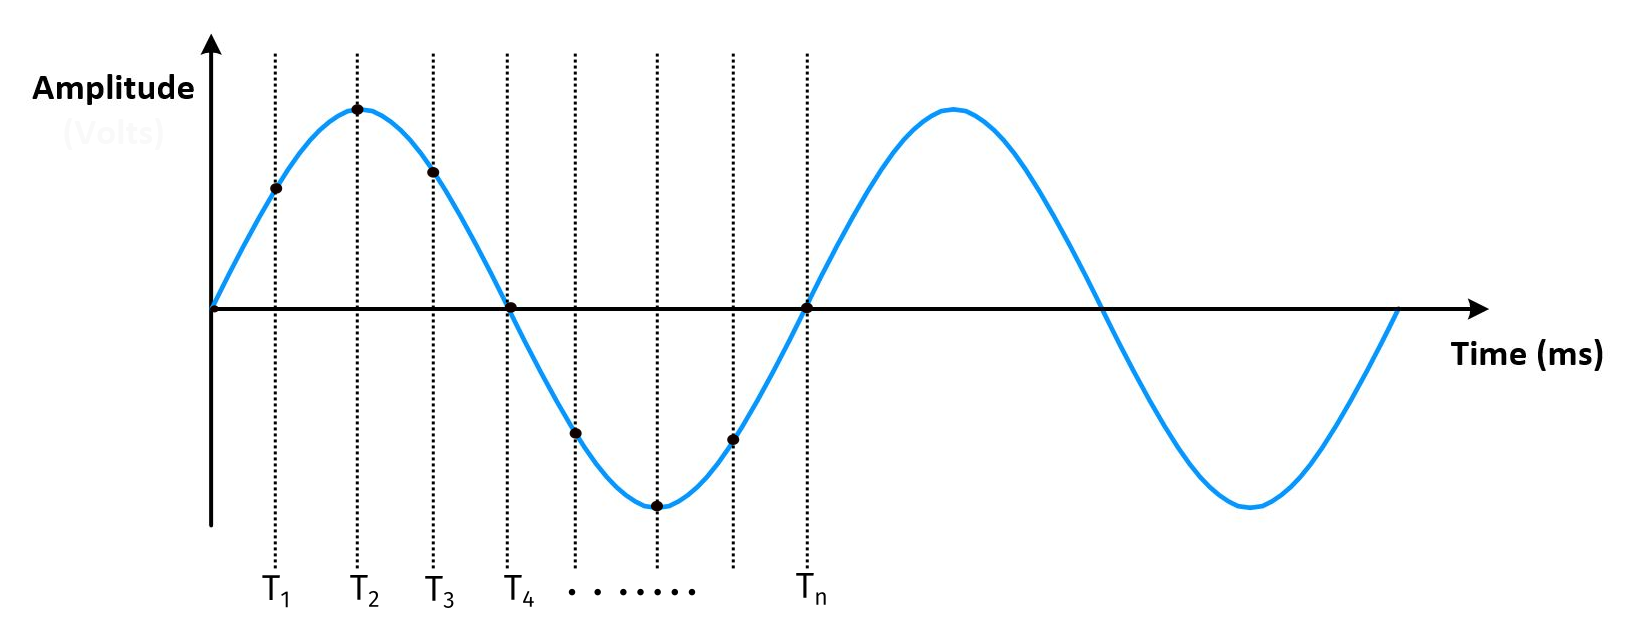
\includegraphics[scale=0.2]{sine_sampled.png} \\
\end{figure}
\pause
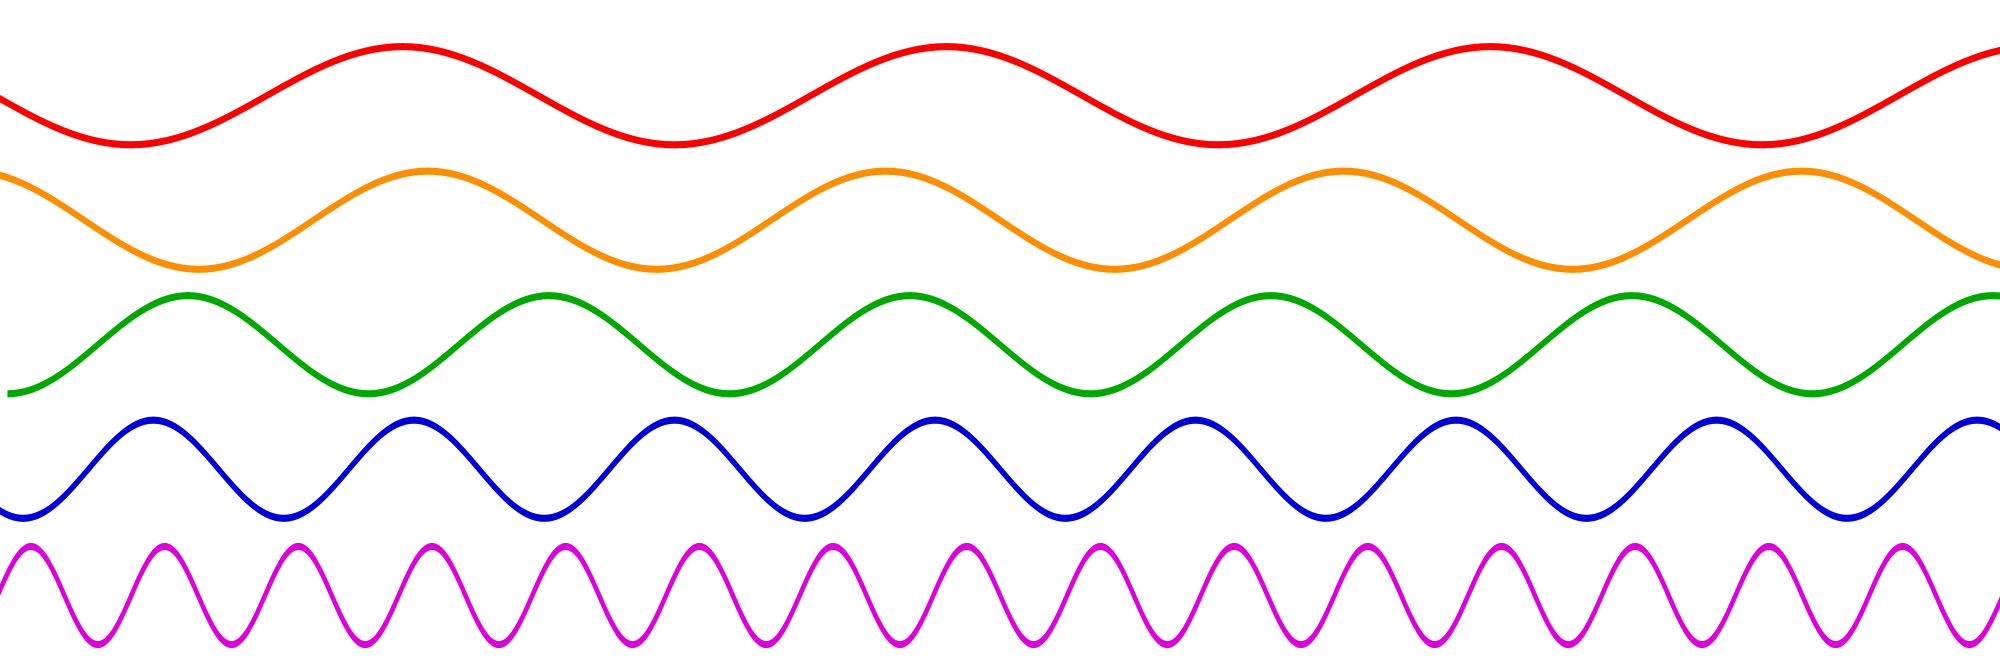
\includegraphics[scale=0.1]{multisine.png}\\
Different make - Incompatibility 
\end{frame}
   %======= Slide Ends ===================
   
   
   %==================================
   \begin{frame}{Total Vector Error}
%   \centering

	\begin{itemize}
	\item Two Quantities to observe - Amplitude \& Phase
	\item Frequency dependency of the result
	\item we require a reference which is  independent and time invarient.
	\item Hence \textbf{Total Vector Error (TVE)} %$^\cite{std:c37}$ 
	\end{itemize}
	$ TVE(n) = \sqrt{\frac{ (\hat{X}_r(n) - X_r(n))^2 + (\hat{X}_i(n)-X_i(n))^2} {X_r(n)^2 + X_i(n)^2}} $ \\
\vspace{5pt}
 \textbf{Type of PMU:}\\
 -Protection  Class: Time critical application, More stringent requirement \\ 
 -Measurement Class: Greater precision not (very) time critical 
   \end{frame}
%=============== Start Slide ===========================
\begin{frame}{Types of Tests}
To get the TVE, compliance test(s) are performed, recommended by C37.118
\begin{enumerate}
\item Steady-state compliance
	\begin{enumerate}
	\item Steady-state synchrophasor measurement requirements
	\item Steady-state frequency and ROCOF measurement requirements
	\end{enumerate}
\item Dynamic compliance
	\begin{enumerate}
	\item Synchrophasor measurement bandwidth requirements using modulated test signals
	\item Ramp of system frequency
	\item Step changes in phase and magnitude
	\end{enumerate}
\end{enumerate} 

\end{frame}

%==================End SLide ===========================   
\section{Literature Survey}

%============= New Slide ============================

\begin{frame}{Literature Survey}
Basically there are 3 components to any arrangement
\begin{itemize}
\item Device Generating Test Signal
\item PMU under test
\item Recording device (PDC etc.)
\end{itemize}

We will See 3 paper here, which are closest to our implementation
\end{frame}

%===================== New Lide
\begin{frame}{paper-1}
Title: \textbf{Dynamic PMU Compliance Test under C37.118.1a-2014} By R. Ghiga
\begin{itemize}
\item Doble F6150 Power System Simulator
\item Three Different PMUs
\item Direct PMU - PSS interfacing
\item Test Performed \cite{Paper:ghiga} : 

\begin{itemize}
	\item Amplitude Modulation: 0.9 - 1.1 PU (\@ 0.1 to 5 Hz)
	\item Phase Modulation: 0.1 rad
	\item Ampli. Step Test: $\pm$ 0.1 PU step
	\item Phase Step Test: 
	\item Freq. Ramp: $\pm$ 1 Hz/s between (44 to 55 Hz)
\end{itemize}

\end{itemize}
IMP: Test signals are \textbf{not} time synchronised.
\end{frame}

%=========== New SLide ===================
\begin{frame}
Title: \textbf{Development of a Smart Grid Test Bed and Applications in PMU and PDC Testing} By Saugata S. B
\begin{itemize}
\item RTDS
\item Multiple Relays/PMU
\item Power Amplifier stanges 
\end{itemize}
\begin{figure}
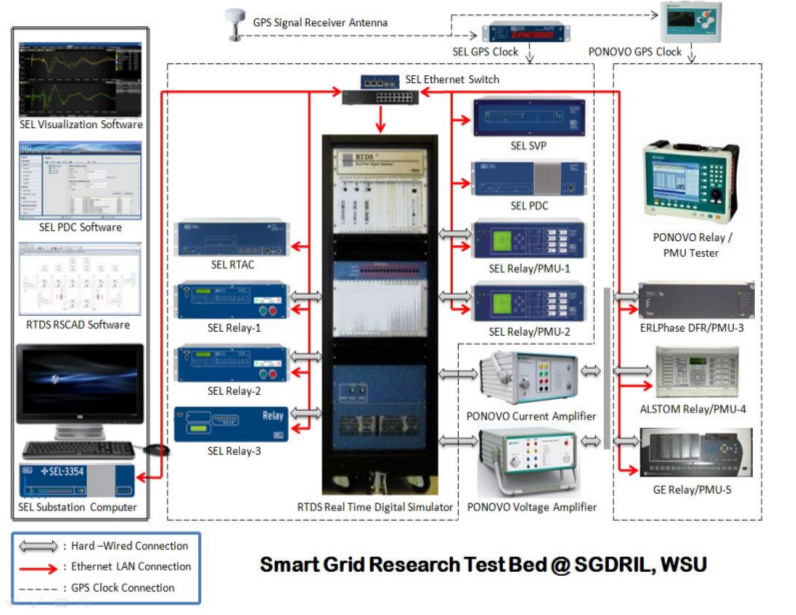
\includegraphics[scale=0.28]{wsu_pmu_setup.png}
\end{figure}
\end{frame}
% ===================== New Slide

\begin{frame}

\end{frame}   

   
    %---------Slide-11 Starts ----------------
    \begin{frame}{References}
\begin{thebibliography}{1}
	\tiny
	%\bibitem{IEEEhowto:kopka}
	%H.~Kopka and P.~W. Daly, \emph{A Guide to \LaTeX}, 3rd~ed.\hskip 1em plus
	%  0.5em minus 0.4em\relax Harlow, England: Addison-Wesley, 1999.
	
	\bibitem{std:c37}
	 C37.118 - IEEE Standard for Synchrophasor Measurements for Power Systems
	
	\bibitem{site:westau}
	http://westernau.com/images/Circle-To-Sine-Wave.png
	
	\bibitem{Book:Phadke}
	Phadke, A.G., Thorp, J.S.,  \textit{Synchronized Phasor Measurements and Their Applications}, Springer US, 2008.
	
	\bibitem{site:ipdc}
	iPDC \& PMU simulator, ipdc.codeplex.com/ 
	\bibitem{Paper:history}
	Phadake A.G., \textit{HISTORY AND APPLICATIONS OF PHASOR MEASUREMENTS}, IEEE, 2006.
	
	
	\bibitem{Paper:ghiga}
	R. Ghiga, Q. Wu, K. Martin, W. Z. El-Khatib, L. Cheng and A. H. Nielsen ``Dynamic PMU Compliance Test under C37.118.1aTM-2014", \textit{IEEE PES GM}, PAge 1-5, 2015
	
	\bibitem{Paper:saugata}
	Saugata S. Biswas, Jeong Hun Kim, Anurag K Srivastava ``Development of a Smart Grid Test Bed and Applications in PMU and PDC Testing", \textit{IEEE Conference Publications}, 2012.	
	

\end{thebibliography}
    \end{frame}
    %---------Slide-11 Ends ----------------


   %---------Slide-4 Starts ----------------
   \begin{frame}
   \begin{center}
   
\includegraphics[scale=0.3]{thanku.png}
   \end{center}
   \end{frame}
      %---------Slide-4 Ends ---------------- 
\end{document}